\section{Proofs}
\label{app:proofs}

\begin{proposition}[valid states]
$\rho_c$ in Eq.~\eqref{eq:state} is positive semi-definite with unit trace. It
is the mixture $\mathbb E_c[\pi(\mathbf z)\psi\psi^{\top}]$ of the encoded pure
states with weights $\pi(\mathbf z)=\|\mathbf v(\mathbf z)\|^2/\mathbb E_c\|\mathbf v\|^2$.
\end{proposition}
\begin{proof}
$\mathbf v\mathbf v^{\top}=\|\mathbf v\|^2\psi\psi^{\top}$. Taking expectations
gives a non-negative combination of rank-one projectors with trace
$\mathbb E_c\|\mathbf v\|^2$.
\end{proof}

\begin{proof}[Proof of Proposition~\ref{prop:unitary}]
$\bar\rho_\delta\mapsto U\bar\rho_\delta U^{\dagger}$. Matrix functions commute
with unitary conjugation, so $E_c\mapsto UE_cU^{\dagger}$ and
$(U\psi)^{\dagger}UE_cU^{\dagger}U\psi=\psi^{\dagger}E_c\psi$.
\end{proof}

\begin{proof}[Proof of Proposition~\ref{prop:shrink}]
$\bar\rho$ and $\bar\rho_\delta$ do not change. Each numerator becomes
$(1-\varepsilon)\psi^{\top}E_c\psi+\varepsilon\psi^{\top}\bar E\psi$ with
$\bar E=\frac1{C_t}\bar\rho_\delta^{-1/2}\bar\rho\,\bar\rho_\delta^{-1/2}$; the
denominator is unchanged. This is one increasing affine map applied to every
class alike.
\end{proof}

\begin{proposition}[scale invariance of the fusion]
For any $a>0$ and class-independent $b(\mathbf z)$, replacing $g_c$ by $a\,g_c+b$
leaves $\hat y$ in Eq.~\eqref{eq:fusion} unchanged.
\end{proposition}
\begin{proof}
$\kappa\mapsto\kappa/a$, so $\kappa g_c\mapsto\kappa g_c+\kappa b/a$, and the added
term does not depend on $c$.
\end{proof}
\noindent Hence the same weight $w$ means the same thing for both sources and on
every dataset, which makes a frozen weight a fair comparison of the PGM and its
twin. For the PGM, the fused softmax is $p_{\mathrm{lin}}(c\mid\mathbf z)\,p(c\mid\mathbf z)^{w\kappa}$
up to normalisation; for integer $k$, $p^k$ is the Born probability of
$E_c^{\otimes k}$ on $k$ copies, so $w\kappa$ acts as an effective number of
measured copies.

\section{Hyper-parameters}
\label{app:hyper}

\begin{table}[h]
\centering
\small
\setlength{\tabcolsep}{2.5pt}
\begin{tabular}{lcccc}
\toprule
 & CIFAR & IN-R & IN-A & CUB \\
\midrule
Epochs, task 0 / later & 10 / 30 & 30 / 30 & 20 / 15 & 20 / 30 \\
Batch size & 64 & 48 & 48 & 128 \\
Learning rate (SGD) & 0.0185 & 0.0067 & 0.0067 & 0.0377 \\
Warm-up epochs & 7 & 4 & 3 & 9 \\
Alignment weight $\beta$ & 1.0 & 3.0 & 3.0 & 1.5 \\
Separation weight & 0.4 & 1.5 & 6.0 & 0.75 \\
Steering weight & 0.2 & 0.5 & 1.0 & 0.2 \\
CosFace scale / margin & 40 / 0.1 & 50 / 0.2 & 30 / 0.3 & 20 / 0.1 \\
Autoencoder code size & 256 & 384 & 128 & 768 \\
Classifier-alignment epochs & 10 & 10 & 10 & 10 \\
\bottomrule
\end{tabular}
\caption{Baseline hyper-parameters (the RSIAT configurations, unchanged).}
\label{tab:hyper}
\end{table}

\paragraph{Components.}
Table~\ref{tab:hyper} lists the baseline settings. The PQK uses 8 qubits, 2
variational layers, one-qubit reduced states, and a bandwidth bounded within a
factor of 10 of the inverse median distance on 512 calibration images. The
PGM uses $\delta=0.1/2^{10}$; the ridge twin $\lambda=0.1\,\mathrm{tr}(\cdot)/d$; the
fusion weight grid is $\{0.25,0.5,1,2,4\}$, with $w=0.25$ (ridge) and $w=0.5$
(PGM) chosen on the tuning group. The Holevo and POVM objectives use a feature
queue of up to 256 images per new class and a weight $\lambda$ calibrated in
the first epoch of task~1 so that the auxiliary gradient norm is half the
classification gradient norm, with a linear warm-up. QKSR-v2 refits the
projection at the start of every task by Fisher LDA on all stored class means
and covariances (ridge $10^{-3}\,\mathrm{tr}(S_W)/d$), scales each projection
row to an angle spread of $0.8$ rad, removes the LayerNorm, and sets $\gamma$ so
that the median kernel between old means and new features is $0.2$.

\section{Per-Task Gap to Joint Training}
\label{app:gap}

\begin{table}[h]
\centering
\small
\setlength{\tabcolsep}{2pt}
\resizebox{\columnwidth}{!}{%
\begin{tabular}{lrrrrrrrrrr}
\toprule
Task & 0 & 1 & 2 & 3 & 4 & 5 & 6 & 7 & 8 & 9\\
\midrule
Joint  & 89.1 & 88.7 & 86.4 & 86.4 & 83.2 & 86.0 & 85.8 & 87.0 & 85.4 & 85.8\\
CIL    & 80.1 & 80.4 & 82.7 & 82.3 & 78.8 & 82.7 & 85.3 & 84.2 & 83.9 & 86.2\\
Oracle & 87.1 & 83.1 & 83.5 & 82.2 & 79.1 & 81.6 & 84.7 & 82.9 & 82.1 & 83.6\\
\midrule
J$-$C & $+9.0$ & $+8.3$ & $+3.7$ & $+4.1$ & $+4.4$ & $+3.3$ & $+0.5$ & $+2.9$ & $+1.6$ & $-0.3$\\
\bottomrule
\end{tabular}}
\caption{Final accuracy (\%) per task on ImageNet-R; task 0 holds the oldest
classes. CIL: baseline, 4 replicates. Oracle: classifier alignment with exact
old-class statistics, 2 runs. Joint: one task with all 200 classes.}
\label{tab:gap}
\end{table}

Table~\ref{tab:gap} gives the per-task values behind Section~\ref{sec:gap}.

\section{Pre-Registered Tests}
\label{app:tests}

\begin{table*}[t]
\centering
\small
\begin{tabular}{llll}
\toprule
Test & Runs & $\Delta$ [95\% CI] & Outcome \\
\midrule
SCF-PGM beats the baseline by $\ge0.3$ $\bar A$, held out & R, A; 8 & $+0.46$ [$+0.28$, $+0.64$] & passed \\
Transfer to unseen datasets, SCF-ridge & CIFAR, CUB; 6 & $+0.11$ [$-0.02$, $+0.24$] & \textbf{failed} \\
Transfer to unseen datasets, SCF-PGM & CIFAR, CUB; 6 & $+0.09$ [$-0.05$, $+0.24$] & \textbf{failed} \\
PGM better than ridge as fusion source & all; 12 & $-0.04$ [$-0.17$, $+0.08$] & \textbf{failed} \\
Oracle states worth $\ge1$ point of $A_B$ & R, A; 11 & $+0.64$ [$+0.48$, $+0.80$] & \textbf{failed} \\
Holevo objective: $A_B$ $\ge+0.5$ over baseline (screening) & R; 1 & $-0.18$ & \textbf{failed}, stopped \\
Holevo + POVM: $A_B$ $\ge+0.5$ over baseline (screening) & R; 1 & $+0.11$ & \textbf{failed}, stopped \\
QKSR: PQK beats RBF twin in $\bar A$ & R; 3 & $+0.07$ [$-0.01$, $+0.15$] & inconclusive \\
QKSR: PQK beats circuit without CNOTs in $\bar A$ & R; 3 & $+0.04$ [$+0.04$, $+0.05$] & passed \\
QKSR-v2: old and new halves up, $\bar A$ CI $>0$ vs QKSR & R; 3 & $-0.07$ [$-0.11$, $-0.03$] & \textbf{failed} \\
Training-time changes stay on the trade-off line (post hoc) & R; 11 & 5 of 5 & held \\
Inference-time changes cross it (post hoc) & R; 9 & $z$ gap $0.83<1$ & \textbf{not met} \\
\bottomrule
\end{tabular}
\caption{Every pre-registered test, in the order it was run.}
\label{tab:tests}
\end{table*}

Table~\ref{tab:tests} lists every pre-registered test with its outcome.

\section{Comparison with Exemplar-Based Methods}
\label{app:exemplar}

\begin{table}[h]
\centering
\small
\setlength{\tabcolsep}{3pt}
\begin{tabular}{lcccc}
\toprule
& \multicolumn{2}{c}{ImageNet-R} & \multicolumn{2}{c}{CIFAR-100} \\
\cmidrule(lr){2-3}\cmidrule(lr){4-5}
Method & $\bar A$ & $A_B$ & $\bar A$ & $A_B$ \\
\midrule
\multicolumn{5}{l}{\textit{Reported by \citet{rsiat}; 20 exemplars per class}} \\
iCaRL~\citep{icarl} & 72.42 & 60.67 & 82.46 & 73.87 \\
DER~\citep{der} & 80.48 & 74.32 & 86.04 & 77.93 \\
FOSTER~\citep{foster} & 81.34 & 74.48 & 89.87 & 84.91 \\
MEMO~\citep{memo} & 74.80 & 66.62 & 84.08 & 75.79 \\
TagFex~\citep{tagfex} & 83.23 & 78.45 & 92.17 & 89.26 \\
\midrule
\multicolumn{5}{l}{\textit{Exemplar-free}} \\
RSIAT, published~\citep{rsiat} & 86.92 & 82.75 & 95.15 & 92.20 \\
RSIAT (ours, 3 seeds) & 87.11 & 82.55 & 95.02 & 92.03 \\
SCF, ridge (ours) & 87.42 & 83.03 & 95.22 & 92.41 \\
SCF, PGM (ours) & 87.50 & 83.07 & 95.23 & 92.34 \\
\bottomrule
\end{tabular}
\caption{Exemplar-based methods with ViT-B/16-IN21K (Table~2 of \citet{rsiat},
authors' partitions, one run) next to exemplar-free results. Our rows use our
partitions and average three seeds.}
\label{tab:exemplar}
\end{table}

Table~\ref{tab:exemplar} shows that, with a pre-trained ViT, the exemplar-free
methods reach higher accuracy than the reported exemplar-based ones on both
benchmarks; the same caveat on partitions as in Table~\ref{tab:main} applies.

\section{Additional Figures}
\label{app:figures}

\begin{figure*}[t]
\centering
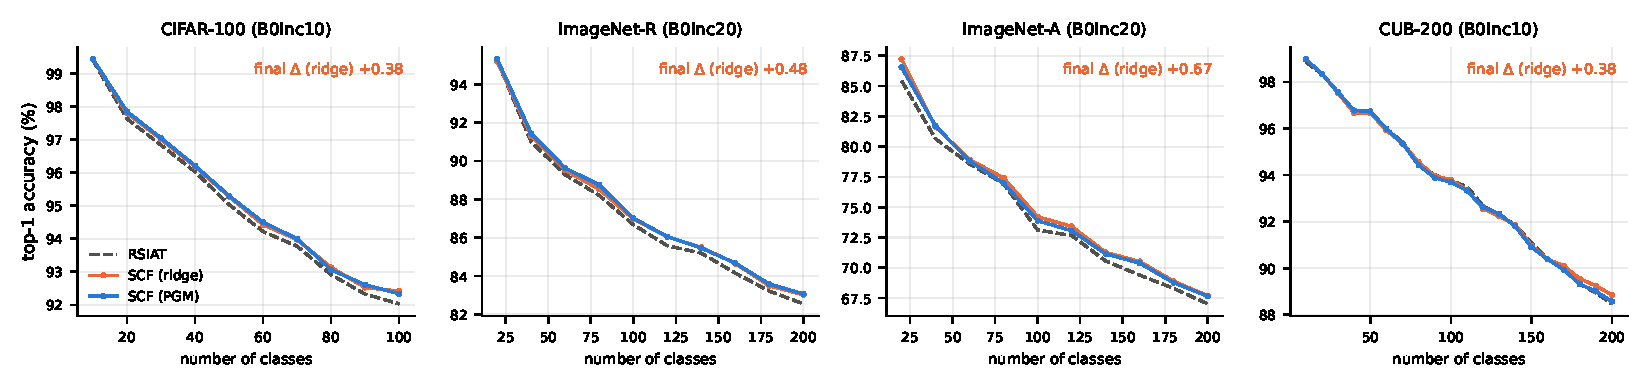
\includegraphics[width=\textwidth]{figures/accuracy_curves.pdf}
\caption{Accuracy after each task against the number of classes seen, mean over
three seeds: RSIAT (ours, dashed) and score fusion with the ridge (orange) and
PGM (blue) sources.}
\label{fig:curves}
\end{figure*}

\begin{figure*}[t]
\centering
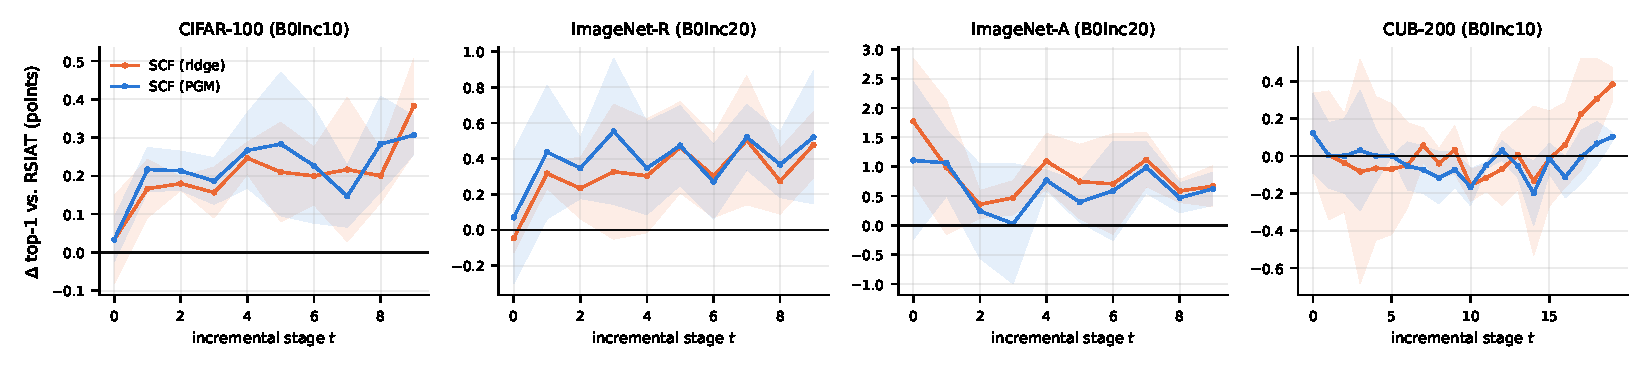
\includegraphics[width=\textwidth]{figures/delta_per_stage.pdf}
\caption{Paired gain of fusion over the baseline at each stage, mean $\pm$ SD
over three seeds. Orange: ridge source (classical). Blue: PGM source (quantum).}
\label{fig:stage}
\end{figure*}

\begin{figure}[t]
\centering
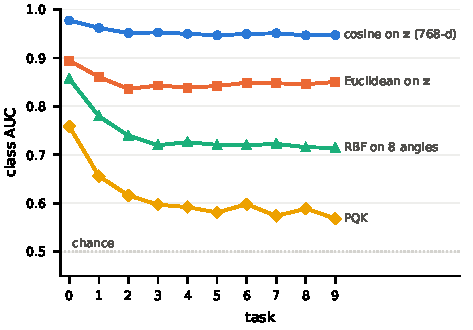
\includegraphics[width=\columnwidth]{figures/probe_auc.pdf}
\caption{Class separability measured by the probe after each task of the QKSR
run (ImageNet-R, seed 1993): probability that a different-class pair is farther
apart than a same-class pair, for distances on the 768-d feature, on the 8
projected angles, and in the PQK.}
\label{fig:probe-auc}
\end{figure}

Figure~\ref{fig:curves} gives the accuracy curves behind Table~\ref{tab:main},
and Figure~\ref{fig:stage} the paired gain of fusion per stage: it is positive
from the second stage on CIFAR-100 and ImageNet-R, largest at the first stage
on ImageNet-A ($+1.8$), and appears only in the last three of 20 stages on
CUB-200. Figure~\ref{fig:probe-auc} traces the probe of Table~\ref{tab:probe}
over tasks: the 768-d feature keeps its class separability, whereas the
separability of the frozen 8-angle projection and of the PQK declines, mostly
within the first three tasks.

\section{Reproducibility}
\label{app:repro}
Configurations, logs, analysis scripts and the specification of every round,
written before the round ran, are in the project repository
\todo{anonymised link}. Every number in this paper is generated from these
files; the probe, its bit-identity test and the trade-off analysis are
included.
